\chapter{Deriving Requirements from Existing Tools}
\label{chap:requirements}

This chapter identifies and analyzes current tools related to OCPM to extract the requirements that our framework must satisfy.
By examining these tools, we gain a clearer understanding of how extensions could be designed.
The resulting requirements are derived from the current tool landscape and from the extensible tools discussed in \cref{chap:related_work}.
These insights form the foundation for the framework design presented in the following chapter.

\section{Systematic Literature Review of Existing Tools}

To identify the framework requirements, a \textit{systematic literature review (SLR)} following \cite{slrguidelines} was conducted.
The review targeted scientific publications related to OCPM and examined the tools introduced within these works.

\subsection{Existing Systematic Literature Reviews}

A recent SLR by Berti et al.\cite{review1} assessed the maturity of OCPM and provided guidance for newcomers to the field. At the time of their study, OCPM was still in an early stage of development. Since then, the field has advanced, most notably with the introduction of the \textit{OCEL 2.0} standard, which was developed to address limitations identified when working with \textit{OCEL 1.0}. For example, it adds explicit object-to-object relations, a feature that was not supported in the original standard and was noted as missing in the earlier review.
Tool support was considered one of the central dimensions of their review. For each analyzed category, the authors highlighted relevant tools and linked them to specific functional areas of OCPM. These categories included the extraction, storage, and preprocessing of object-centric event data, as well as process discovery, conformance checking, and performance analysis.

While tool support was discussed in their review, it was not analyzed in the level of detail required for this thesis. Berti et al.\ also identified persistent challenges, such as usability issues and compatibility problems, which are still relevant when assessing current tools. Since their study, the field has further evolved, which increases the need for a more comprehensive analysis that focuses directly on the research tools themselves.

\subsection{Search Method}
To identify recent research tools in OCPM, an SLR was conducted using Scopus, applying the terms \textit{object-centric} and \textit{process mining} to titles, abstracts, and keywords.
Earlier abbreviations such as \textit{artifact-centric} or \textit{object-aware} were not included, as OCPM has since matured and become standardized.
Adding domain-specific terms (e.g., \textit{process discovery}, \textit{conformance checking}) did not yield additional results and was therefore omitted.
The publication period was restricted to January 2020 to October 2025, as the release of the \textit{OCEL 1.0} standard \cite{ocel1}, marked the beginning of standardized research in OCPM.
The applied methodology, including the query and filters, is summarized in Figure~\ref{fig:slrprocess}.
Applying these restrictions resulted in an initial set of 127 search results before applying exclusion criteria.

\begin{figure}[htbp]
	\centering
	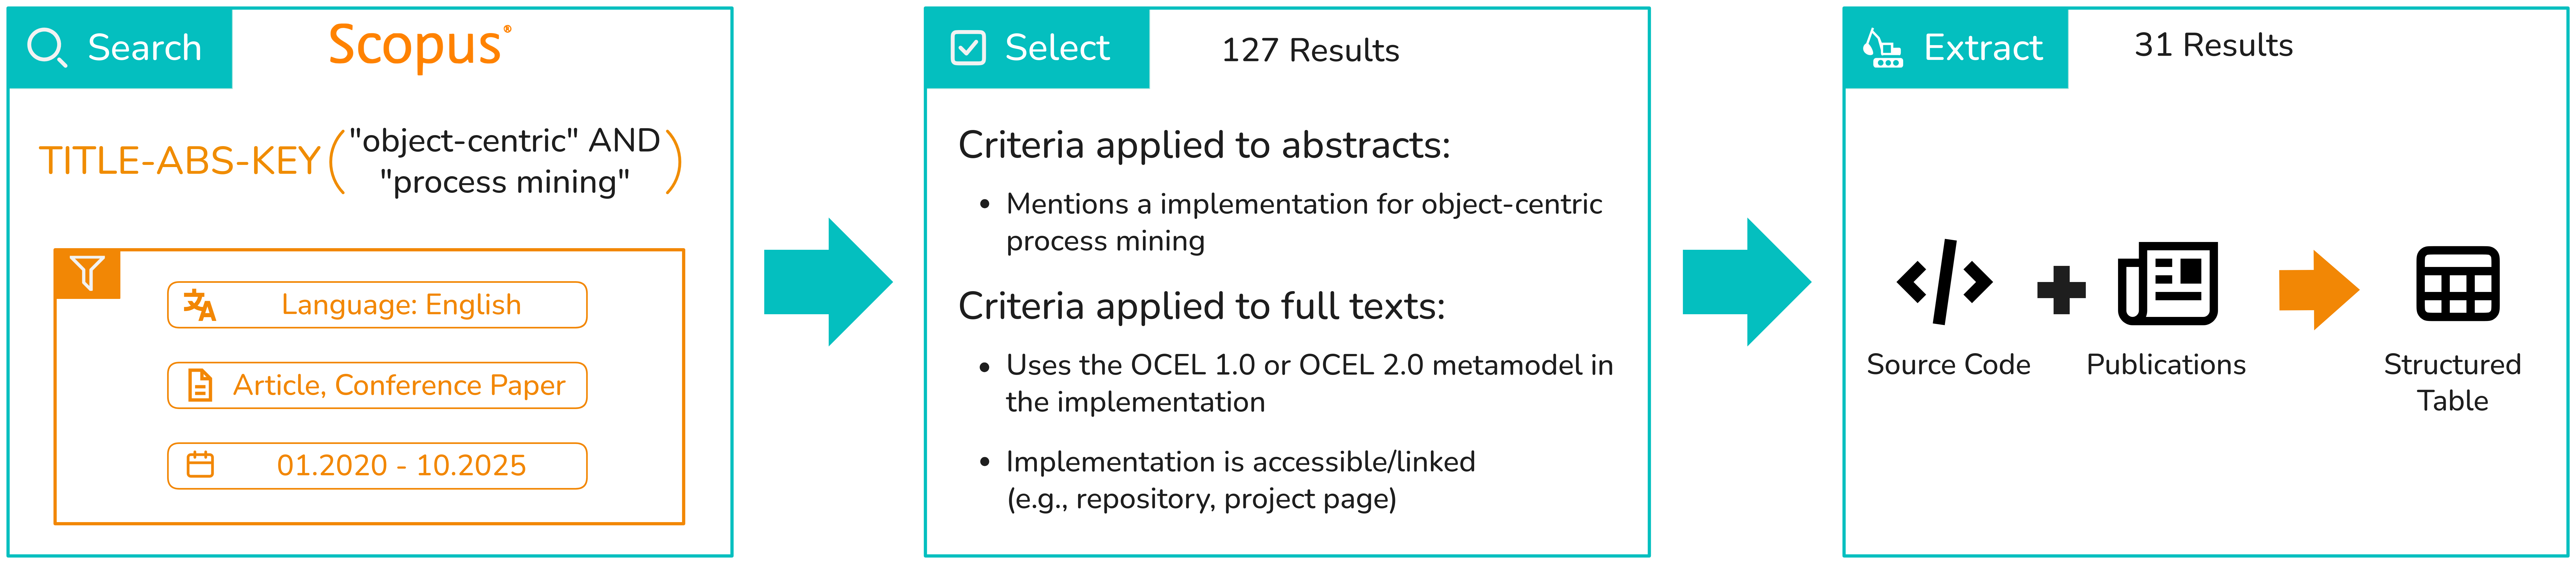
\includegraphics[width=\textwidth]{figures/slr/SLR.png}
	\caption{Systematic literature review process, including search query, filters, and exclusion criteria.}
	\label{fig:slrprocess}
\end{figure}

\subsection{Exclusion Criteria}
A publication was excluded if the abstract did not meet the following criteria:

\begin{itemize}
	\item It explicitly mentioned object-centric process mining.
	\item It indicated either a tool, an implementation, or an evaluation of the proposed technique.
\end{itemize}

During the full-text screening, two additional requirements were applied:

\begin{itemize}
	\item The publication had to rely on the \textit{OCEL 1.0} or \textit{OCEL 2.0} meta-model. Works using alternative data structures, such as event knowledge graphs, were excluded.
	\item The publication had to provide access to the referenced tool or implementation, for example through a repository or project page.
\end{itemize}

Papers that mentioned a tool in the abstract but did not provide an accessible implementation were removed. For example, \cite{casenotion} and \cite{ocprocesstrees} describe approaches without accessible tool support and were therefore excluded.

\subsection{Extraction}
From the 31 included publications, both the papers and the referenced tools were examined.
Whenever possible, the tools were downloaded, inspected, and tested.
If a released version was available, it was recorded; otherwise, the commit number or download date was noted.
Open-source projects were briefly checked at code level, and installation was attempted by following the documentation or, if missing, common practices.
All extracted information was captured in a structured table.
A short overview of the extracted tools is shown in Table~\ref{tab:tool-overview}, while the complete table with all details is provided in Appendix~\ref{app:tools}.

\begin{sidewaystable}[p]
	\caption{Overview of analyzed tools (detailed version in Appendix~\ref{app:tools}).}
	\label{tab:tool-overview}
	\small
	\centering
	\begin{tabular}{|l|p{4cm}|l|p{2cm}|l|l|p{4.5cm}|}
		\hline
		Ref                       & Name                             & Type         & Standard             & Language            & Operational & Category                                               \\ \hline
		\cite{oclpm}              & ObjectCentricLPMs                & ProM Plugin  & OCEL 1.X             & java                & No          & Discovery                                              \\ \hline
		\cite{constraintchecking} & ObjectCentric-ConstraintChecking & ProM Plugin  & OCEL 1.X             & java                & No          & Constraint Checking                                    \\ \hline
		\cite{olap}               & processmining                    & Library      & OCEL 2.0             & python              & Yes         & Discovery,  Transformation                             \\ \hline
		\cite{rust4pm}            & Rust4PM                          & Library      & OCEL 2.0             & rust                & Yes         & Extraction                                             \\ \hline
		\cite{pm4py}              & PM4Py                            & Library      & OCEL 2.0             & python              & Yes         & Extraction, Discovery, Filtering                       \\ \hline
		\cite{ocpa}               & ocpa                             & Library      & OCEL 1.X             & python              & No          & Extraction, Discovery, Performance, Conformance        \\ \hline
		\cite{ocel2}              & pm4js                            & Library      & OCEL 2.0             & javascript          & Yes         & Extraction, Filtering                                  \\ \hline
		\cite{ocpm}               & OC-PM                            & Hosted       & OCEL 2.0             & javascript          & Yes         & Extraction, Filtering, Discovery, Conformance          \\ \hline
		\cite{ocel2}              & Ocelot                           & Hosted       & OCEL 2.0             & typescript          & Yes         & Inspection                                             \\ \hline
		\cite{ocpq}               & OCPQ                             & GUI          & OCEL 2.0             & rust, typescript    & Yes         & Discovery,  Filtering, Inspection, Constraint Checking \\ \hline
		\cite{qrpm}               & QRPM                             & GUI          & OCEL 2.0 + Extension & python              & Yes         & Extraction, Filtering, Discovery, Inspection           \\ \hline
		\cite{oxminer}            & OX Miner                         & GUI          & OCEL 2.0             & python, typescript  & No          & Root Cause Analysis                                    \\ \hline
		\cite{proact}             & ProAct                           & GUI          & OCEL 2.0             & python, typescript  & No          & Constraint Checking                                    \\ \hline
		\cite{ocpsm}              & OCPS                             & GUI          & OCEL 1.X             & python, typescript  & No          & Simulation                                             \\ \hline
		\cite{propp}              & ProPPa                           & GUI          & OCEL 1.X             & python              & No          & Conformance                                            \\ \hline
		\cite{ocpi}               & OC$\pi$                          & GUI          & OCEL 2.0             & closed source       & Yes         & Discovery, Variant Analysis                            \\ \hline
		\cite{opera}              & OPerA                            & GUI          & OCEL 1.X             & python,  typescript & No          & Performance                                            \\ \hline
		\cite{occnet}             & Object-Centric Causal Net Miner  & CLI / WebApp & OCEL 2.0             & python,  typescript & No          & Discovery                                              \\ \hline
		\cite{ethereum}           & trace\_based\_logging            & CLI          & OCEL 2.0             & python              & No          & Extraction                                             \\ \hline
		\cite{aoe}                & aoe2PM                           & CLI          & OCEL 2.0             & python              & Yes         & Extraction                                             \\ \hline
		\cite{textmining}         & OCEL-extractor                   & CLI          & OCEL 2.0             & python              & Yes         & Extraction                                             \\ \hline
		\cite{omop}               & omop2ocel                        & CLI          & OCEL 2.0             & python              & Yes         & Extraction                                             \\ \hline
		\cite{graphnn}            & DAEiOcBPvGNN                     & CLI          & OCEL 1.X             & python              & No          & Machine Learning                                       \\ \hline
		\cite{ococomot}           & oCoCoMoT                         & CLI          & OCEL 1.X             & python              & No          & Conformance                                            \\ \hline
		\cite{ocdm}               & ObjectCentricDCR                 & CLI          & OCEL 1.X             & typescript          & Yes         & Discovery                                              \\ \hline
		\cite{silentobjects}      & BPM\_2024\_Silent\_Objects       & CLI          & OCEL 1.X             & python              & Yes         & Discovery                                              \\ \hline
		\cite{supervariants}      & Super Variants                   & CLI          & OCEL 1.X             & python              & No          & Variant Analysis                                       \\ \hline
		\cite{mmlpm}              & PreservingOCStructures           & CLI          & OCEL 1.X             & python              & ~           & Machine Learning                                       \\ \hline
		\cite{alignments}         & object-centric-alignments        & CLI          & OCEL 1.X             & python              & Yes         & Conformance                                            \\ \hline
		\cite{precfit}            & PrecisionFitnessOCPM             & CLI          & OCEL 1.X             & python              & No          & Conformance                                            \\ \hline
		\cite{totem}              & TOTeM                            & CLI          & OCEL 2.0             & python              & Yes         & Discovery                                              \\ \hline
	\end{tabular}
\end{sidewaystable}

\subsection{Technical Analysis of Existing Tools}

Before defining the technical requirements, the tools identified through the systematic literature review were analyzed to understand the technologies, implementation choices, and design approaches currently used in OCPM. This analysis gives an overview of the current technical landscape and forms the basis for deriving the framework requirements.
Table~\ref{tab:tech-analysis-tools-summary} summarizes the main observations for each analyzed aspect, which are discussed in more detail in the following paragraphs.

\begin{table}[H]
	\centering
	\small
	\setlength{\tabcolsep}{6pt}
	\renewcommand{\arraystretch}{1.15}
	\begin{tabularx}{\linewidth}{lX}
		\toprule
		\textbf{Category}               & \textbf{Summary}                                                                                                               \\
		\midrule
		\textbf{Programming Languages}  & Python is the primary language for OCPM, with Rust emerging for performance-sensitive implementations.                         \\
		\textbf{Libraries}              & Only Python libraries go beyond basic import/export, but they are still incomplete or unreliable.                              \\
		\textbf{CLI Tools}              & CLI tools are primarily research prototypes with substantial setup effort and limited reusable outputs.                        \\
		\textbf{Implementation of GUIs} & GUIs are implemented as ProM plugins or web applications, with most being web-based.                                           \\
		\textbf{GUIs}                   & Compared to CLI tools, GUIs improve usability through interactive, OCPM-specific inputs and visualizations.                    \\
		\textbf{Filtering}              & Filtering is commonly used in OCPM tools to support OCPM tasks; most approaches focus on basic filtering operations.           \\
		\textbf{Inspection}             & GUIs commonly provide basic OCEL inspection (tables, summary statistics) to support OCPM analysis decisions.                   \\
		\textbf{Process Models}         & Most tools use object-centric adaptations of case-centric notations as process models for output, input, and visualization.    \\
		\textbf{Interoperability}       & Interoperability is largely limited to OCEL exchange; process models and other artifacts remain tool-specific.                 \\
		\textbf{Installation and Setup} & Installation is often challenging due to missing documentation, fragile dependencies, and the lack of packaging or installers. \\
		\textbf{Extensibility}          & Most tools are not designed for extension, which leads to repeated reimplementation of common functionality.                   \\
		\bottomrule
	\end{tabularx}
	\caption{Summary of the technical analysis of existing OCPM tools}
	\label{tab:tech-analysis-tools-summary}
\end{table}

\paragraph{Programming Languages.}

The analyzed tools use several programming languages, each serving different purposes:

\begin{itemize}
	\item \textbf{Python} is the dominant language and is used in 23 tools. Its popularity is mainly due to the strong data science and process mining ecosystem.

	\item \textbf{TypeScript and JavaScript} are mostly used to build user interfaces for web applications. An exception is \textit{ObjectCentricDCR}~\cite{ocdm}, where the mining logic itself is implemented entirely in TypeScript.

	\item \textbf{Rust} has recently entered the field as a high-performance alternative to traditional languages. In OCPM, it is used to build standalone tools such as the process mining library \textit{Rust4PM}~\cite{rust4pm} and the \textit{OCPQ} tool~\cite{ocpq}, and to accelerate existing ecosystems through language bindings. For example, the \textit{rustxes}\footnote{\url{https://pypi.org/project/rustxes}} package provides a Python interface for Rust-based OCEL import functions, allowing users to benefit from Rust’s speed within the Python ecosystem.
	\item \textbf{Java} appears only in the \textit{ProM} framework~\cite{ocpm, oclpm,constraintchecking}, where it is used for developing plugins.
\end{itemize}

\begin{figure}[htbp]
	\centering
	\begin{tikzpicture}
		\pie[text=legend, radius=2, color={blue!40, orange!50, green!50, red!50, gray!40}]
		{74/Python, 13/JavaScript \& TypeScript, 6/Rust, 6/Java, 3/Unknown}
	\end{tikzpicture}
	\caption{Distribution of programming languages used by tools implementing their process mining functionality.}
	\label{fig:language_distribution}
\end{figure}


\paragraph{Libraries.}

Process mining libraries form the foundation of nearly all process mining tools. As shown in Table~\ref{tab:ocpm-libraries}, each of the main programming languages has at least one available library. However, only the Python-based libraries go beyond basic import and export functions and simple OCEL statistics such as activity names, frequencies, and object counts.

\begin{table}[H]
	\centering
	\caption{Overview of main libraries used for object-centric process mining. Symbols indicate support (\cmark), partial support (\kmark), or lack of support (\xmark).}
	\label{tab:ocpm-libraries}
	\small
	\begin{tabular}{|l|l|c|c|c|c|c|c|c|}
		\hline
		\textbf{Library}                       & \textbf{Language} &
		\rotatebox{90}{\textbf{Import/Export}} &
		\rotatebox{90}{\textbf{Discovery}}     &
		\rotatebox{90}{\textbf{Conformance}}   &
		\rotatebox{90}{\textbf{Performance}}   &
		\rotatebox{90}{\textbf{Filtering}}     &
		\rotatebox{90}{\textbf{Statistics}}    &
		\rotatebox{90}{\textbf{Maintained}}                                                                                       \\ \hline

		\textit{PM4Py}~\cite{pm4py}            & Python            & \cmark & \cmark & \kmark & \xmark & \cmark & \cmark & \cmark \\ \hline
		\textit{OCPA}~\cite{ocpa}              & Python            & \cmark & \cmark & \cmark & \cmark & \xmark & \xmark & \xmark \\ \hline
		\textit{Rust4PM}~\cite{rust4pm}        & Rust              & \cmark & \xmark & \xmark & \xmark & \xmark & \xmark & \cmark \\ \hline
		\textit{PM4JS}~\cite{ocel2}            & JavaScript        & \cmark & \xmark & \xmark & \xmark & \xmark & \cmark & \cmark \\ \hline
	\end{tabular}
\end{table}

\textit{PM4Py}~\cite{pm4py} is a general-purpose process mining library that has gradually been extended to support object-centric concepts.
It provides utilities for importing and exporting OCEL data and includes discovery functions such as directly-follows graphs and Petri nets.
However, these features still originate from case-centric designs.
For example, the implemented object-centric Petri nets create separate Petri nets for each flattened object type rather than a single integrated model.
This approach is similar to how object-centric directly-follows graphs are handled.
Conformance checking is available only as part of the discovery process and not as a separate analysis step.

\textit{OCPA}~\cite{ocpa} was developed specifically for object-centric process mining.
It supports all major analysis categories, including discovery, conformance, and performance analysis, and introduces key concepts such as object variants, process executions, and object-centric conformance measures.
These features go beyond the functionality offered by \textit{PM4Py}.
Despite this broader coverage, the library faces several challenges.
The documentation is limited and unstructured, which makes it difficult to locate specific functionality, and the overall package structure is difficult to use.
It also appears to no longer be actively maintained.
For example, common \textit{OCEL~2.0} logs cannot be imported, an issue that has been known for quite some time\footnote{\url{https://github.com/ocpm/ocpa/issues/19}} but has not been resolved.

Although all of these libraries contribute to the development of object-centric process mining, none provide a complete and practical solution.
There is still no single library that fully supports object-centric process mining in a comprehensive and reliable way.

\paragraph{Command-Line-Based Tools.}

Thirteen of the 31 tools identified in the analysis are implemented as command-line applications without a graphical user interface. These tools are typically used as single-purpose scripts or lightweight libraries. Users either modify example scripts and execute them directly~\cite{totem}, adjust configuration files before running the tool, or pass parameters through the command line~\cite{ococomot}.

This design choice is understandable, as implementing a graphical interface often requires more effort than developing the core process mining functionality. At the same time, the prevalence of command-line tools highlights a broader issue: there is no common platform for integrating new object-centric algorithms into a user-friendly environment. The \textit{ProM} framework~\cite{prom}, which historically played this role for case-centric process mining, is not widely used for OCPM, and only two dedicated plugins exist.

In many cases, developing a full application is either not considered worthwhile or requires expertise that is not available. A representative example is the \textit{Object-Centric Causal Net Miner}~\cite{occnet}. Mining is initiated through a Python script that requires manual input of the log path and parameters. Once executed, the script launches a minimal web viewer to display the discovered model. This design serves as a pragmatic workaround to avoid the additional complexity of implementing full import, export, and interaction features.

Most command-line tools function as proof-of-concept implementations or algorithmic benchmarks rather than practical end-user tools. For instance, \textit{BPM\_2024\_Silent\_Objects}~\cite{silentobjects} outputs only the number of discovered silent objects, and \textit{TOTeM}~\cite{totem} prints the mined model as console text without providing it as a structured result. Such designs make further analysis or integration difficult without modifying the source code.

A significant portion of the command-line tools can be classified as \textit{extractors} that transform domain-specific data into OCEL. Examples include tools for processing blockchain transactions~\cite{ethereum}, healthcare data~\cite{omop}, or textual sources~\cite{textmining}. While these extractors provide useful entry points for their respective domains, they can be challenging to use in practice, especially for domain experts who may lack the technical knowledge required to adapt scripts and configuration files manually.

\paragraph{Implementation of Graphical Interfaces.}

Graphical user interfaces in object-centric process mining tools are implemented using three main approaches:

\begin{itemize}
	\item \textbf{ProM plugins.}
	      These interfaces are integrated directly into the ProM framework~\cite{prom, oclpm, constraintchecking}.
	      They are written in Java and follow the conventions of the ProM environment.
	\item \textbf{Python-based interfaces using Dash.}
	      These tools rely entirely on Python and commonly use the \textit{Dash}\footnote{\url{https://dash.plotly.com/}} framework to build simple, self-contained applications~\cite{qrpm, ocpm}.
	      While they can be developed and maintained with only Python knowledge, they are often limited in interactivity and scalability.
	\item \textbf{Web-based applications.}
	      These tools are implemented as standard web applications in TypeScript or JavaScript and can use the large ecosystem of frameworks such as \textit{React}\footnote{\url{https://react.dev/}}, \textit{Angular}\footnote{\url{https://angular.dev/}}, or \textit{Vue}\footnote{\url{https://vuejs.org/}}. Most of them run locally and rely on a dedicated backend written in Python or Rust to perform the process mining tasks, while the frontend handles user interaction and visualization.
	      A smaller number of tools are deployed as hosted websites in which the browser performs both the interaction layer and the process mining computations. This is achieved with technologies such as Rust bindings compiled to WebAssembly~\cite{rust4pm} or the \textit{PM4JS} library. While this approach allows the tool to run entirely in the browser, it also limits the available process mining functionality.
	      Web-based applications offer high flexibility and interactivity, but they also require more technical expertise to develop and maintain.
\end{itemize}

\paragraph{Graphical User Interfaces.}

Several of the analyzed tools provide graphical user interfaces (GUIs), offering a more user-friendly and accessible experience compared to command-line applications. Most GUI-based tools implement basic functionality such as importing and exporting OCEL files, providing an overview of the loaded log, and supporting limited filtering operations. Some tools, such as \textit{OC-PM}~\cite{ocpm}, are designed as general-purpose applications and are frequently used in case studies of object-centric process mining~\cite{casestudy1}. Others introduce GUIs to make specific object-centric techniques easier to apply through interactive inputs.

Input forms replace manual configuration file editing and provide structured fields for parameter specification. These inputs often include standard parameters such as the name of the process discovery algorithm variant or checkboxes for enabling additional computations, for example in performance analyses~\cite{opera}. More advanced tools offer specialized input mechanisms. In \textit{OCPQ}, for example, users can define custom code fragments using the Common Expression Language, while numeric parameters can be adjusted with sliders to simplify experimentation.

A particularly useful class of input elements are those populated dynamically from the loaded log. These fields adapt to the log’s structure and expose its attributes for configuration. Common examples include selection fields for activities or object types, as seen in \textit{OC$\pi$}, where users can choose which object types should be considered during variant mining or which activity should serve as the leading event when computing process executions. In some cases, such as \textit{OX Miner}~\cite{oxminer}, input options are derived from computations on the log itself. For instance, predicates can be generated automatically from the uploaded log and then combined into custom analytical formulas.

Constraint-checking tools form another category of GUI-based systems~\cite{ocpq, proact, constraintchecking}. In these tools, assumptions about process behavior are modeled graphically as constraint graphs and checked against the uploaded log, either for querying and filtering~\cite{ocpq} or for detecting constraint violations~\cite{proact}. These systems often include interactive graph builders in which constraints are defined through nodes and edges with embedded input fields. In \textit{ProAct}, the constraint graph is relatively simple: nodes represent activities or object types and are connected through edges, with small forms used to specify metrics and thresholds. More advanced implementations, such as \textit{OCPQ}, include nodes representing collections of filters, variable definitions, and multiple constraints that can be combined to form complete queries.

The outputs of GUI-based tools vary depending on their purpose and level of complexity. Many tools present results as process models visualized as graphs, either as static images~\cite{ocpi} or as interactive diagrams with selectable nodes and edges~\cite{opera}. Some tools focus on variant visualizations~\cite{ocpi}, while others, such as \textit{ProAct} and \textit{OCPQ}, provide interactive views for exploring analytical results~\cite{proact, ocpq}. In some cases, the output is a single value, for example the percentage of process executions that satisfy a given constraint~\cite{ocpq}. Other tools export new OCEL files that can be used for further analysis~\cite{ocpq}.



\paragraph{Process Models.}

Process models are formal representations of how a process is executed and form a central component of almost all object-centric process mining tools. Most of the models identified in the analyzed tools are adaptations of existing case-centric notations. Common examples include object-centric Petri nets~\cite{ocpi, pm4py, ocpa}, object-centric directly-follows graphs~\cite{proact, pm4py}, object-centric Dynamic Condition Response (DCR) graphs~\cite{ocdm}, and object-centric causal nets~\cite{occnet}.

Some tools extend these adapted formalisms to capture object-centric behavior more effectively. For example, \textit{QRPM}~\cite{qrpm} extends object-centric Petri nets into \textit{Quantity Nets} to represent quantity-related processes, while \textit{Silent Objects}~\cite{silentobjects} introduces the concept of silent objects, which are groups of synchronized objects shared across multiple activities. The only identified model that does not originate from a case-centric notation is the model introduced by \textit{TOTeM}~\cite{totem}.

Process models in object-centric process mining tools are used for several purposes:
\begin{enumerate}[label=\arabic*., leftmargin=1.2cm]
	\item \textbf{As the main output of the tool.}
	      Many tools produce process models as their primary result, either to present a new model type or to demonstrate a discovery method, as seen in \textit{TOTeM}~\cite{totem}, \textit{Object-Centric Local Process Models}~\cite{oclpm}, and object-centric causal nets~\cite{occnet}.

	\item \textbf{As input for further analysis.}
	      Process models are also used as inputs for other techniques. For instance, \textit{Object-Centric Alignments}~\cite{alignments} takes an OCPN as input for performing conformance checking.

	\item \textbf{To provide an overview for decision-making.}
	      Some tools visualize process models to help users understand the underlying event log and support analytical decisions. In \textit{ProAct}~\cite{proact}, for example, an object-centric directly-follows graph is generated to identify operational constraints that are later expressed as constraint graphs.

	\item \textbf{To visualize and annotate analytical results.}
	      In several tools, process models serve as visual layers for highlighting metrics or relationships. \textit{OX Miner}~\cite{oxminer} embeds mined association rules within a directly-follows graph, while \textit{OPerA}~\cite{opera} overlays performance measures on an object-centric Petri net.

	\item \textbf{As interactive interfaces.}
	      Some tools allow users to interact directly with the process model. For example, in \textit{OC-PM}~\cite{ocpm}, users can explore and filter related objects and relations by interacting with an object-centric Petri net.
\end{enumerate}

All tools that visualize object-centric process models represent them using graph-based structures. While the specific notation differs across tools, the visual conventions are similar. Nodes typically represent activities or object-related states, and edges express causal or behavioral relations. These graphs are often annotated to support interpretation. For example, edges may show frequencies or waiting times, as in the directly-follows graph of \textit{ProAct}~\cite{proact}, and nodes may display event counts, as in the object-centric Petri net of \textit{OC-PM}~\cite{ocpm}. Many tools also support interactive elements that allow users to inspect additional information, such as statistics or performance metrics, by selecting nodes or edges.

\paragraph{Filtering.}
Filtering is a common feature in OCPM tools. It is either implemented directly within the tool, as in \textit{OC-PM}~\cite{ocpm} and \textit{QRPM}~\cite{qrpm}, which provide advanced filtering options, or it appears indirectly through input parameters. For example, in \textit{OC$\pi$}~\cite{ocpi}, users can include or exclude specific object types during variant computation, effectively using input fields as filters.

Several tools support filtering through visual feedback. \textit{QRPM}, for instance, displays pie charts showing object counts per type to help users select relevant object types, while \textit{Ocelot}~\cite{ocel2} visualizes event distributions over time to assist in defining time-based filters.

In other cases, filtering is not implemented within the tool itself but is described only as a preprocessing step in the corresponding publication. For example, in~\cite{oxminer}, the authors report excluding objects of one type when they are related to multiple objects of another type.

Overall, while filtering is an essential step in OCPM, its implementation varies widely across tools and is not yet handled consistently in existing interfaces.

\paragraph{Inspection.}

Another functionality implemented in nearly all tools with a graphical interface is the inspection of the underlying event log.
In most cases, except for \textit{Ocelot}~\cite{ocel2}, inspection is not the main purpose of the tool but supports users in making decisions for the primary analysis task.

Inspection features often include general statistics such as counts of object types or activities.
These statistics may be visualized as charts, as in \textit{OC-PM}~\cite{ocpm}, or displayed as simple numeric summaries, as in \textit{Ocelot}.
Some tools also provide structural views inspired by UML, such as cards summarizing attribute information or diagrams that illustrate object relations~\cite{ocel2,ocpq}.

A common additional feature is the ability to export inspection views as images, allowing users to reuse them in documentation or research publications.


\paragraph{Interoperability Between Tools}

Another notable observation is that none of the analyzed tools are interoperable beyond the exchange of OCEL files. While OCELs generated by one tool can usually be used in another, other types of data, particularly process models, cannot be shared easily between tools. At present, there is no common exchange format for object-centric process models. A partial exception is found in \textit{oCoCoMoT}~\cite{ococomot}, where Petri nets are stored using the PNML format, although the notation for colored Petri nets is repurposed to represent object types as colors, following the idea proposed by van der Aalst~\cite{processdiscovery}.

This lack of interoperability has several consequences. First, most process models exist only within the tools that generate them and cannot be reused for further analyses, such as conformance checking in systems like \textit{object-centric-alignments}~\cite{alignments}. Second, it leads to duplicated computation efforts, since models must be rediscovered rather than imported or exchanged. Third, reproducibility becomes more difficult. Many command-line tools serve as references for experiments, and if they depend on external process mining libraries that evolve over time, their results may become inconsistent or impossible to replicate.


\paragraph{Installation and Setup}

Installation and setup remain major challenges for most object-centric process mining tools. Nearly all tools are distributed as standalone applications that must be installed and configured individually. The only exceptions are web-hosted tools such as \textit{Ocelot} and \textit{OC-PM}~\cite{ocpm}, which can be accessed directly through a web browser without any local setup. However, these tools must be actively hosted and maintained by their developers, which limits their long-term availability.

Convenient installers are rare. \textit{OCPQ} is the only tool that provides installers for all major operating systems, while \textit{OC$\pi$} offers an installer exclusively for Windows with no alternative installation method. All other tools require manual installation, which often demands considerable technical knowledge.

Even when installation instructions are available, running the tools can be difficult due to several recurring issues:

\begin{enumerate}[label=\arabic*., leftmargin=1.2cm]
	\item \textbf{Missing or incomplete instructions.}
	      Some tools lack installation documentation altogether~\cite{supervariants}, while others provide only partial guidance~\cite{ocpsm}. In several cases, developers assume the use of a specific package manager or environment, which forces users into the same setup.

	\item \textbf{Unspecified or missing dependencies.}
	      Certain tools rely on external libraries without clearly stating which ones~\cite{oxminer, supervariants}, or list dependencies without version pinning, which often leads to incompatibilities~\cite{aoe}.

	\item \textbf{Broken or unreliable dependency management.}
	      Even when dependencies are pinned, installation can still fail due to outdated packages or conflicting version requirements~\cite{proact, opera}.

	\item \textbf{Complex or system-dependent requirements.}
	      Some tools depend on additional components that must be installed manually, such as the Yices or Z3 solvers used in \textit{oCoCoMoT}~\cite{ococomot}, or the Graphviz bindings required by \textit{QRPM}. These dependencies vary in difficulty across operating systems and further complicate installation.
\end{enumerate}

Because of these issues, many tools are effectively unusable for non-technical users. The situation is made more difficult by the fact that most tools are no longer actively maintained after their initial release, which leaves compatibility problems unresolved over time.

\paragraph{Extensibility}

Most command-line tools, as discussed earlier, are not particularly user-friendly. At the same time, developing a complete graphical interface requires significant effort that is unrelated to the core process mining functionality and demands frontend development knowledge that many data scientists do not have.

As discussed in \cref{chap:related_work}, the \textit{ProM} framework successfully addressed this issue for case-centric process mining. However, it is not used in the current OCPM tool landscape.

Using existing OCPM tools as a base for further development is also not feasible. These tools were never designed to be extended, and most have unorganized project structures. Setting up the development environment often requires substantial effort, and documentation is frequently missing or incomplete, with a few exceptions such as \textit{ProAct} and \textit{OCPQ}~\cite{proact, ocpq}. As a result, many codebases appear to have been written as research prototypes rather than reusable software systems. Developing a user-friendly tool therefore often requires starting from scratch or investing significant effort into restructuring existing projects.

Even small functionalities that could theoretically be reused across tools lack general-purpose implementations. For example, visualizing object-centric Petri nets must be reimplemented for every new tool. Existing tools such as \textit{OC-PM}, \textit{OCPS}, \textit{OPerA}, and \textit{OC$\pi$} each contain their own custom visualization based on different libraries, none of which can be reused or integrated easily into new tools.

This is particularly problematic because graph layouting and visualization are not trivial tasks. Configuring general-purpose layout libraries often requires extensive manual adjustment and still produces suboptimal results. Object-centric process models, in particular, may require specialized layouting algorithms to achieve meaningful and readable visualizations~\cite{dfglayouting}.

\section{Deriving Framework Requirements}
\label{sec:requirements}

The systematic literature review and the technical analysis revealed recurring challenges in current OCPM tools. These challenges include limited extensibility, missing interoperability standards, inconsistent visualization approaches, and low usability.

Based on these findings and on the analysis of the tools discussed in \cref{chap:related_work}, we derive requirements for the base tool itself, as well as requirements for two different ways of extending it:

\begin{itemize}
	\item \textbf{External Extensions:} Extensions that use Ocelescope as an environment for running OCPM functions. They are loaded after the compilation of the tool, similar to plugins in ProM.
	\item \textbf{Embedded Extensions:} Extensions that use Ocelescope as a foundation for building custom OCPM tools. This approach results in specialized tools that reuse Ocelescope’s core functionality.
\end{itemize}

We introduce these mechanisms to reflect the current tool landscape: external extensions primarily target lightweight research tools by providing a reliable way to package and execute them within Ocelescope, whereas embedded extensions primarily target applications that require specialized interaction and visualization while avoiding the need to reimplement recurring infrastructure.

The derived requirements are listed in \autoref{tab:requirements} and serve as the basis for the framework design presented in the following chapter.

\begin{table}[t]
	\centering
	\small
	\caption{Requirements for the Ocelescope framework}
	\label{tab:requirements}
	\renewcommand{\arraystretch}{1.15}

	\begin{tabularx}{\textwidth}{|S|A|R|I|}
		\hline
		\textbf{Scope} & \textbf{Aspect}                                                      & \textbf{Requirement}                                      & \textbf{ID} \\ \hline

		% ================= Base Functionality =================
		\scoperow[-0.8ex]{11}{Base Functionality \ \ \ }
		               & \multirow{2}{*}{OCEL management}
		               & Import and export of standard OCEL formats                           & BF-1a                                                                   \\ \cline{3-4}
		               &                                                                      & Support for extensions to OCELs                           & BF-1b       \\ \cline{2-4}

		               & \multirow{2}{*}{Graphical user interface}
		               & Adaptive interface across different display sizes                    & BF-2a                                                                   \\ \cline{3-4}
		               &                                                                      & Consistent appearance across operating systems            & BF-2b       \\ \cline{2-4}

		               & \multirow{2}{*}{Filtering}
		               & Provision of commonly used OCEL filters                              & BF-3a                                                                   \\ \cline{3-4}
		               &                                                                      & Interactive definition of filters                         & BF-3b       \\ \cline{2-4}

		               & Inspection
		               & Support for inspection and exploration of OCELs                      & BF-4                                                                    \\ \cline{2-4}

		               & \multirow{4}{*}{Usability}
		               & Robustness (dependency and versioning)                               & BF-5a                                                                   \\ \cline{3-4}
		               &                                                                      & Few system dependencies                                   & BF-5b       \\ \cline{3-4}
		               &                                                                      & Simple and concise setup process                          & BF-5c       \\ \cline{3-4}
		               &                                                                      & Usable by non-technical users                             & BF-5d       \\ \hline

		% ================= External Extensions =================
		\scoperow[-0.8ex]{13}{External Extensions \ \ \ \ }
		               & Integration
		               & Integration into the main interface without recompilation or restart & EX-1                                                                    \\ \cline{2-4}

		               & \multirow{3}{*}{Artifact definition}
		               & Automatic exchange format for artifacts                              & EX-2a                                                                   \\ \cline{3-4}
		               &                                                                      & Cross-compatibility between extensions                    & EX-2b       \\ \cline{3-4}
		               &                                                                      & Support for nested and annotated artifacts                & EX-2c       \\ \cline{2-4}

		               & \multirow{3}{*}{Artifact visualization}
		               & Support for a broad range of visualization types                     & EX-3a                                                                   \\ \cline{3-4}
		               &                                                                      & Support for nested visualizations                         & EX-3b       \\ \cline{3-4}
		               &                                                                      & Export of visualizations in common formats                & EX-3c       \\ \cline{2-4}

		               & \multirow{2}{*}{Function user interface}
		               & Automatic generation of a graphical user interface                   & EX-4a                                                                   \\ \cline{3-4}
		               &                                                                      & Input fields that adapt dynamically based on other inputs & EX-4b       \\ \cline{2-4}

		               & Developer experience
		               & Minimal introduction of additional abstractions                      & EX-5                                                                    \\ \cline{2-4}

		               & Function implementation
		               & Implemented in Python or Rust                                        & EX-6                                                                    \\ \cline{2-4}

		               & Documentation
		               & Extensive and accessible documentation                               & EX-7                                                                    \\ \hline

		% ================= Embedded Extensions =================
		\scoperow[-0.8ex]{8}{Embedded Extensions \ \ }
		               & User interface implementation
		               & Implementation using established web frameworks                      & EM-1                                                                    \\ \cline{2-4}

		               & OCPM implementation
		               & Implemented in Python or Rust                                        & EM-2                                                                    \\ \cline{2-4}

		               & \multirow{2}{*}{Modularity}
		               & Support for isolated and reusable extensions                         & EM-3a                                                                   \\ \cline{3-4}
		               &                                                                      & Encouragement of modular extension design                 & EM-3b       \\ \cline{2-4}

		               & \multirow{2}{*}{Developer experience}
		               & Close to the implementation style of established frameworks          & EM-4a                                                                   \\ \cline{3-4}
		               &                                                                      & Extensive and accessible documentation                    & EM-4b       \\ \cline{2-4}

		               & \multirow{2}{*}{Integration}
		               & Integration through an automated build process                       & EM-5a                                                                   \\ \cline{3-4}
		               &                                                                      & Clear entry points for extension development              & EM-5b       \\ \hline
	\end{tabularx}
\end{table}
